\documentclass[12pt,letterpaper,fleqn]{hmcpset}
\usepackage[margin=1in]{geometry}
\usepackage{graphicx}
\usepackage{amsmath,amssymb}
\usepackage{enumerate}
\usepackage{hyperref}
\usepackage{parskip}
\usepackage{listings}

% Theorems
\usepackage{amsthm}
\renewcommand\qedsymbol{$\blacksquare$}
\makeatletter
\@ifclassloaded{article}{
    \newtheorem{definition}{Definition}[section]
    \newtheorem{example}{Example}[section]
    \newtheorem{theorem}{Theorem}[section]
    \newtheorem{corollary}{Corollary}[theorem]
    \newtheorem{lemma}{Lemma}[theorem]
}{
}
\makeatother

% Random Stuff
\setlength\unitlength{1mm}

\newcommand{\insertfig}[3]{
\begin{figure}[htbp]\begin{center}\begin{picture}(120,90)
\put(0,-5){\includegraphics[width=12cm,height=9cm,clip=]{#1.eps}}\end{picture}\end{center}
\caption{#2}\label{#3}\end{figure}}

\newcommand{\insertxfig}[4]{
\begin{figure}[htbp]
\begin{center}
\leavevmode \centerline{\resizebox{#4\textwidth}{!}{\input
#1.pstex_t}}
\caption{#2} \label{#3}
\end{center}
\end{figure}}

\long\def\comment#1{}

\newcommand\norm[1]{\left\lVert#1\right\rVert}
\DeclareMathOperator*{\argmin}{arg\,min}
\DeclareMathOperator*{\argmax}{arg\,max}

% bb font symbols
\newfont{\bbb}{msbm10 scaled 700}
\newcommand{\CCC}{\mbox{\bbb C}}

\newfont{\bbf}{msbm10 scaled 1100}
\newcommand{\CC}{\mbox{\bbf C}}
\newcommand{\PP}{\mbox{\bbf P}}
\newcommand{\RR}{\mbox{\bbf R}}
\newcommand{\QQ}{\mbox{\bbf Q}}
\newcommand{\ZZ}{\mbox{\bbf Z}}
\renewcommand{\SS}{\mbox{\bbf S}}
\newcommand{\FF}{\mbox{\bbf F}}
\newcommand{\GG}{\mbox{\bbf G}}
\newcommand{\EE}{\mbox{\bbf E}}
\newcommand{\NN}{\mbox{\bbf N}}
\newcommand{\KK}{\mbox{\bbf K}}
\newcommand{\KL}{\mbox{\bbf KL}}

% Vectors
\renewcommand{\aa}{{\bf a}}
\newcommand{\bb}{{\bf b}}
\newcommand{\cc}{{\bf c}}
\newcommand{\dd}{{\bf d}}
\newcommand{\ee}{{\bf e}}
\newcommand{\ff}{{\bf f}}
\renewcommand{\gg}{{\bf g}}
\newcommand{\hh}{{\bf h}}
\newcommand{\ii}{{\bf i}}
\newcommand{\jj}{{\bf j}}
\newcommand{\kk}{{\bf k}}
\renewcommand{\ll}{{\bf l}}
\newcommand{\mm}{{\bf m}}
\newcommand{\nn}{{\bf n}}
\newcommand{\oo}{{\bf o}}
\newcommand{\pp}{{\bf p}}
\newcommand{\qq}{{\bf q}}
\newcommand{\rr}{{\bf r}}
\renewcommand{\ss}{{\bf s}}
\renewcommand{\tt}{{\bf t}}
\newcommand{\uu}{{\bf u}}
\newcommand{\ww}{{\bf w}}
\newcommand{\vv}{{\bf v}}
\newcommand{\xx}{{\bf x}}
\newcommand{\yy}{{\bf y}}
\newcommand{\zz}{{\bf z}}
\newcommand{\0}{{\bf 0}}
\newcommand{\1}{{\bf 1}}

% Matrices
\newcommand{\Ab}{{\bf A}}
\newcommand{\Bb}{{\bf B}}
\newcommand{\Cb}{{\bf C}}
\newcommand{\Db}{{\bf D}}
\newcommand{\Eb}{{\bf E}}
\newcommand{\Fb}{{\bf F}}
\newcommand{\Gb}{{\bf G}}
\newcommand{\Hb}{{\bf H}}
\newcommand{\Ib}{{\bf I}}
\newcommand{\Jb}{{\bf J}}
\newcommand{\Kb}{{\bf K}}
\newcommand{\Lb}{{\bf L}}
\newcommand{\Mb}{{\bf M}}
\newcommand{\Nb}{{\bf N}}
\newcommand{\Ob}{{\bf O}}
\newcommand{\Pb}{{\bf P}}
\newcommand{\Qb}{{\bf Q}}
\newcommand{\Rb}{{\bf R}}
\newcommand{\Sb}{{\bf S}}
\newcommand{\Tb}{{\bf T}}
\newcommand{\Ub}{{\bf U}}
\newcommand{\Wb}{{\bf W}}
\newcommand{\Vb}{{\bf V}}
\newcommand{\Xb}{{\bf X}}
\newcommand{\Yb}{{\bf Y}}
\newcommand{\Zb}{{\bf Z}}

% Calligraphic
\newcommand{\Ac}{{\cal A}}
\newcommand{\Bc}{{\cal B}}
\newcommand{\Cc}{{\cal C}}
\newcommand{\Dc}{{\cal D}}
\newcommand{\Ec}{{\cal E}}
\newcommand{\Fc}{{\cal F}}
\newcommand{\Gc}{{\cal G}}
\newcommand{\Hc}{{\cal H}}
\newcommand{\Ic}{{\cal I}}
\newcommand{\Jc}{{\cal J}}
\newcommand{\Kc}{{\cal K}}
\newcommand{\Lc}{{\cal L}}
\newcommand{\Mc}{{\cal M}}
\newcommand{\Nc}{{\cal N}}
\newcommand{\Oc}{{\cal O}}
\newcommand{\Pc}{{\cal P}}
\newcommand{\Qc}{{\cal Q}}
\newcommand{\Rc}{{\cal R}}
\newcommand{\Sc}{{\cal S}}
\newcommand{\Tc}{{\cal T}}
\newcommand{\Uc}{{\cal U}}
\newcommand{\Wc}{{\cal W}}
\newcommand{\Vc}{{\cal V}}
\newcommand{\Xc}{{\cal X}}
\newcommand{\Yc}{{\cal Y}}
\newcommand{\Zc}{{\cal Z}}

% Bold greek letters
\newcommand{\alphab}{\hbox{\boldmath$\alpha$}}
\newcommand{\betab}{\hbox{\boldmath$\beta$}}
\newcommand{\gammab}{\hbox{\boldmath$\gamma$}}
\newcommand{\deltab}{\hbox{\boldmath$\delta$}}
\newcommand{\etab}{\hbox{\boldmath$\eta$}}
\newcommand{\lambdab}{\hbox{\boldmath$\lambda$}}
\newcommand{\epsilonb}{\hbox{\boldmath$\epsilon$}}
\newcommand{\nub}{\hbox{\boldmath$\nu$}}
\newcommand{\mub}{\hbox{\boldmath$\mu$}}
\newcommand{\zetab}{\hbox{\boldmath$\zeta$}}
\newcommand{\phib}{\hbox{\boldmath$\phi$}}
\newcommand{\psib}{\hbox{\boldmath$\psi$}}
\newcommand{\thetab}{\hbox{\boldmath$\theta$}}
\newcommand{\taub}{\hbox{\boldmath$\tau$}}
\newcommand{\omegab}{\hbox{\boldmath$\omega$}}
\newcommand{\xib}{\hbox{\boldmath$\xi$}}
\newcommand{\sigmab}{\hbox{\boldmath$\sigma$}}
\newcommand{\pib}{\hbox{\boldmath$\pi$}}
\newcommand{\rhob}{\hbox{\boldmath$\rho$}}

\newcommand{\Gammab}{\hbox{\boldmath$\Gamma$}}
\newcommand{\Lambdab}{\hbox{\boldmath$\Lambda$}}
\newcommand{\Deltab}{\hbox{\boldmath$\Delta$}}
\newcommand{\Sigmab}{\hbox{\boldmath$\Sigma$}}
\newcommand{\Phib}{\hbox{\boldmath$\Phi$}}
\newcommand{\Pib}{\hbox{\boldmath$\Pi$}}
\newcommand{\Psib}{\hbox{\boldmath$\Psi$}}
\newcommand{\Thetab}{\hbox{\boldmath$\Theta$}}
\newcommand{\Omegab}{\hbox{\boldmath$\Omega$}}
\newcommand{\Xib}{\hbox{\boldmath$\Xi$}}

% mixed symbols
\newcommand{\sinc}{{\hbox{sinc}}}
\newcommand{\diag}{{\hbox{diag}}}
\renewcommand{\det}{{\hbox{det}}}
\newcommand{\trace}{{\hbox{tr}}}
\newcommand{\tr}{\trace}
\newcommand{\sign}{{\hbox{sign}}}
\renewcommand{\arg}{{\hbox{arg}}}
\newcommand{\var}{{\hbox{var}}}
\newcommand{\cov}{{\hbox{cov}}}
\renewcommand{\Re}{{\rm Re}}
\renewcommand{\Im}{{\rm Im}}
\newcommand{\eqdef}{\stackrel{\Delta}{=}}
\newcommand{\defines}{{\,\,\stackrel{\scriptscriptstyle \bigtriangleup}{=}\,\,}}
\newcommand{\<}{\left\langle}
\renewcommand{\>}{\right\rangle}
\newcommand{\Psf}{{\sf P}}
\newcommand{\T}{\top}
\newcommand{\m}[1]{\begin{bmatrix} #1 \end{bmatrix}}

% info for header block in upper right hand corner
\name{Nathaniel Diamant}
\class{Math 189r}
\assignment{Homework 2}
\duedate{October 10, 2016}

\begin{document}

There are 6 problems in this set. You need to do 3 problems (due in class on Monday)
every week for 2 weeks. Note that this means you must eventually complete all problems.
Feel free to work with other students, but make sure you write up the homework
and code on your own (no copying homework \textit{or} code; no pair programming).
Feel free to ask students or instructors for help debugging code or whatever else,
though.
When implementing algorithms you may not use any library (such as \texttt{sklearn})
that already implements the algorithms but you may use any other library for
data cleaning and numeric purposes (\texttt{numpy} or \texttt{pandas}). Use common
sense. Problems are in no specific order.\\[1em]

\textbf{1. (Conditioning a Gaussian)} Note that from Murphy page 113. ``Equation 4.69
is of such importance in this book that we have put a box around it, so you can easily
find it.'' That equation is important. Read through the proof of the result.
Suppose we have a distribution over random variables $\xx = (\xx_1, \xx_2)$ that is
jointly Gaussian with parameters
\[
    \mub = \m{\mub_1\\\mub_2}\;\;\; \Sigmab = \m{\Sigmab_{11}&\Sigmab_{12}\\\Sigmab_{21}&\Sigmab_{22}},
\]
where
\[
    \mub_1 = \m{0\\0}, \;\; \mub_2 = 5, \;\; \Sigmab_{11} = \m{6 & 8\\ 8 & 13}, \;\; \Sigmab_{21}^\T = \Sigmab_{12} = \m{5\\11}, \;\; \Sigmab_{22} = \m{14}.
\]
Compute
\begin{enumerate}[(a)]
    \item The marginal distribution $p(\xx_1)$. Plot the density in $\RR^2$.
    \item The marginal distribution $p(\xx_2)$. Plot the density in $\RR^1$.
    \item The conditional distribution $p(\xx_1 | \xx_2)$
    \item The conditional distribution $p(\xx_2 | \xx_1)$\\[1em]
\end{enumerate}

\begin{solution}
    \begin{enumerate}[(a)]
        \item
            From Murphy: 
            \begin{align*}
                 p(\xx_1) &= \Nc(\xx_1|\mub_1, \Sigma_{11}) \\
                 &= \Nc \left(\xx_1|\m{0\\0}, \m{6 & 8\\ 8 & 13} \right)
             \end{align*} 
             Which we can make a 2-d density plot of in numpy.\\
             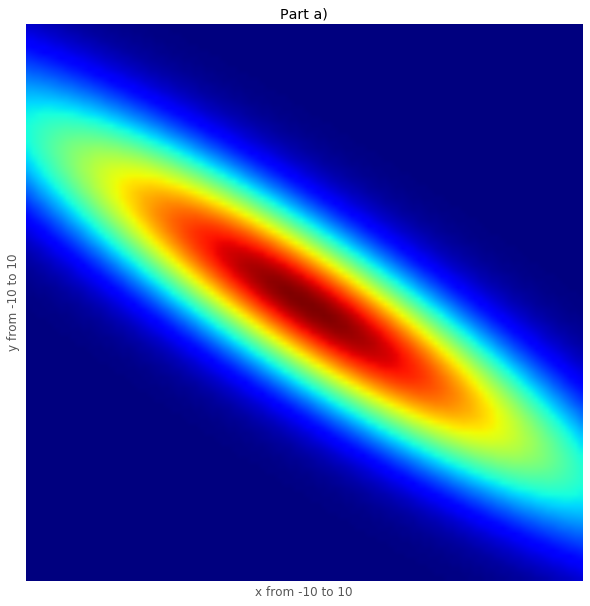
\includegraphics[scale = .5]{p1a.png}
        \item
            Similarly: 
            \begin{align*}
                p(x_2) &= \Nc(x_2|\mu_2, \Sigma_2) \\
                 &= \Nc \left(x_2|5, 14 \right)
            \end{align*}
            Which we can make a 2-d density plot of in numpy.\\
            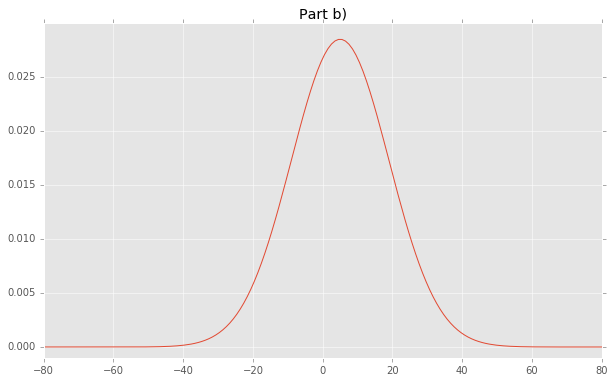
\includegraphics[scale = .5]{p1b.png}
        \item
            The conditional distribution, $p(\xx_1 | x_2)$, is found,
            $$
                p(\xx_1 | x_2) = \Nc(\mub_{1|2}, \Sigma_{1|2})\\
            $$
            where,
            \begin{align*}
                \mub_{1|2} &= \mub_1 + \Sigma_{12} \Sigma_{22}^{-1}(x_2 - \mu_2) \\
                 &= \m{0\\0} + \m{5\\11} \m{14}^{-1} (x_2 - 5)\\
                 &= \m{\frac{5}{14}\\\frac{11}{14}}(x_2 - 5)
            \end{align*}
            and
            \begin{align*}
                \Sigma_{1|2} &= \Sigma_{11} - \Sigma_{12}\Sigma_{22}\Sigma_{21}\\
                &= \m{6 & 8\\ 8 & 13} - \m{5\\11} \m{14}^{-1} \m{5 & 11}\\
                &= \m{\frac{59}{14} & \frac{57}{14} \\ \frac{57}{14} & \frac{61}{14} }\\
            \end{align*}
            So,
            $$  p(\xx_1 | \xx_2) = \Nc \left(\xx_1 | \m{\frac{5}{14}\\\frac{11}{14}}(x_2 - 5), \m{\frac{59}{14} & \frac{57}{14} \\ \frac{57}{14} & \frac{61}{14} } \right) $$
        \item
            The conditional distribution, $p(x_2 | \xx_1)$, is found,
            $$
                p(x_2 | \xx_1) = \Nc(\mu_{2|1}, \Sigma_{2|1})\\
            $$
            where,
            \begin{align*}
                \mu_{2|1} &= \mu_2 + \Sigma_{21} \Sigma_{11}^{-1}(\xx_1 - \mub_1) \\
                &= 5 + \m{5 & 11} \m{6 & 8\\ 8 & 13}^{-1} (\xx_1 - \m{0\\0})\\
                &= 5 + \m{-\frac{23}{14} & \frac{13}{7}}\xx_1
            \end{align*}
            and
            \begin{align*}
                \Sigma_{2|1} &= \Sigma_{22} - \Sigma_{21}\Sigma_{11}\Sigma_{12}\\
                &= 14 - \m{5 & 11} \m{6 & 8\\ 8 & 13} \m{5 \\ 11} \\
                &= \frac{25}{14}              
            \end{align*}
            So, 
            $$ p(x_2 | \xx_1) = \Nc \left( x_2 | 5 + \m{-\frac{23}{14} & \frac{13}{7}}\xx_1, \frac{25}{14} \right) $$
    \end{enumerate}
\end{solution}

\textbf{2. ($\ell_1$-Regularization)} Consider the $\ell_1$ norm of a vector $\xx\in\RR^n$:
\[
    \|\xx\|_1 = \sum_i |\xx_i|.
\]
Plot the norm-ball $B_k = \{\xx : \|\xx\|_1 \leq k\}$ for $k=1$. On the same plot, plot
the Euclidean norm-ball $A_k = \{\xx : \|\xx\|_2 \leq k\}$ for $k=1$ behind the first plot.
Show that the optimization problem
\begin{align*}
    \text{minimize: } & f(\xx)\\
    \text{subj. to: } & \|\xx\|_p \leq k
\end{align*}
is equivalent to
\begin{align*}
    \text{minimize: } & f(\xx) + \lambda\|\xx\|_p
\end{align*}
(hint: create the Lagrangian). With this knowledge, and the plots given above, argue why
using $\ell_1$ regularization (adding a $\lambda\|\xx\|_1$ term to the objective) will give
sparser solutions than using $\ell_2$ regularization for suitably large $\lambda$.\\[1em]

Our plot in 2 dimensions:\\\\
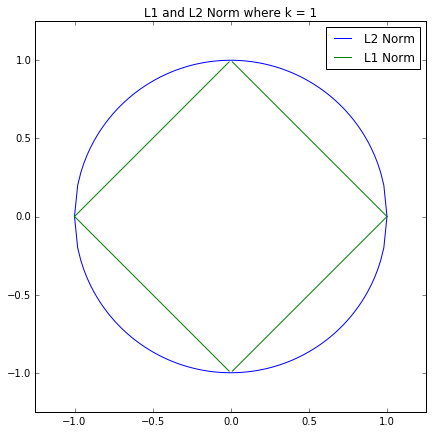
\includegraphics[scale = .5]{p2.png}\\

We will begin by constructing the Lagrangian.
\begin{align*}
     \text{minimize: } & f(\xx) \\
     \text{subj. to: } & \|\xx\|_p \leq k \\
     \text{Is equivalent to}\\    
     \underset{x}{\min}\underset{\lambda \geq 0}{\max} & f(x) + \lambda(\norm{x}_p - k) \\
\end{align*}
Now that we have the Lagrangian, we can construct the dual. 
\begin{align*}
    \underset{\lambda \geq 0}{\max} \underset{x}{\min}& f(x) + \lambda(\norm{x}_p - k) \\
    \underset{\lambda \geq 0}{\max} \underset{x}{\min}& f(x) + \lambda \norm{x}_p - \lambda k \\
\end{align*}
Note that $\lambda k$ is a constant under the minimization of $x$, so the problem becomes:
    $$\underset{\lambda \geq 0}{\max}  \underset{x}{\min} f(x) + \lambda \norm{x}_p$$
Which, when solving for $x*$, is equivalent to 
\begin{align*}
    \text{minimize: } & f(\xx) + \lambda\|\xx\|_p
\end{align*}
As desired. The dual is equivalent to the original problem ubder Slater's conditions assuming $f(x)$ is convex, because the contraint is clearly convex and feasible. \\\\

One reason that the L1-norm encourages sparser solutions is that compared to the L2 norm, it punishes terms close to zero much more harshly. We can see this in the dual problem, because as $x$ approaches zero in $\norm{x}_2$, $x**2$ approaches zero much more quickly than the absolute value of $x$.


\textbf{3. (Lasso)} Show that placing an equal zero-mean Laplace prior on each element of the weights $\thetab$
of a model is equivelent to $\ell_1$ regularization in the Maximum-a-Posteriori estimate
\begin{align*}
    \text{maximize: } & \PP(\thetab | \Dc) = \frac{\PP(\Dc | \thetab)\PP(\thetab)}{\PP(\Dc)}.
\end{align*}
Note the form of the Laplace distribution is
\[
    \mathrm{Lap}(x|\mu,b) = \frac{1}{2b}\exp\left(-\frac{|x-\mu|}{b}\right)
\]
where $\mu$ is the location parameter and $b>0$ controls the variance. Plot the density
$\mathrm{Lap}(x|0,1)$ and the standard normal $\Nc(x|0,1)$ and suggest why this would
lead to sparser solutions than a Gaussian prior on each elements of the weights
(which correspond to $\ell_2$ regularization).\\[1em]

\vspace{10mm}

\textbf{4. (Lasso Feature Selection)} Ignoring undifferentiability at $x=0$, take $\frac{\partial |x|}{\partial x}
= \mathrm{sign} (x)$. Using this, show that $\nabla \|\xx\|_1 = \mathrm{sign}(\xx)$ where $\mathrm{sign}$ is applied
elementwise. Derive the gradient of the $\ell_1$ regularized linear regression objective
\begin{align*}
    \text{minimize: } & \|A\xx - \bb\|_2^2 + \lambda \|\xx\|_1
\end{align*}
Now consider the shares dataset we used in problem 1 of homework 1
(\url{https://math189r.github.io/hw/data/online_news_popularity/online_news_popularity.txt}).
Implement a gradient descent based solution of the above optimization problem for this data. Produce
the convergence plot (objective vs. iterations) for a non-trivial value of $\lambda$.
In the same figure (and different axes) produce a `regularization path' plot. Detailed
more in section 13.3.4 of Murphy, a regularization path is a plot of the optimal weight on
the $y$ axis at a given regularization strength $\lambda$ on the $x$ axis. Armed with this
plot, provide an ordered list of the top five features in predicting the log-shares of a news
article from this dataset (with justification). We can see a more detailed analysis of this
at \url{https://en.wikipedia.org/wiki/Proximal_gradient_methods_for_learning} and
\url{https://web.stanford.edu/~boyd/papers/pdf/prox_algs.pdf} but you will have to wrap
the gradient descent step with a threshold function
\[
    \mathrm{prox}_{\gamma}(\xx)_i = \begin{cases}
        \xx_i - \gamma & \xx_i > \gamma\\
        0 & |\xx_i| \leq \gamma\\
        \xx_i + \gamma & x_i < -\gamma
    \end{cases}
\]
so that each iterate
\[
    \xx_{i+1} = \mathrm{prox}_{\gamma}\left( \xx_i - \gamma \nabla f(\xx_i) \right)
\]
where $\gamma$ is your learning rate. Tip: you can reuse most of your code from the
first homework.\\[1em]

\textbf{5. (SVD Image Compression)} Load the image of a scary clown at \url{http://i.imgur.com/X017qGH.jpg}
into a matrix/array. Plot the progression of the 100 largest singular values for the original image
and a randomly shuffled version of the same image (all on the same plot). In a single figure plot
a grid of four images: the original image, and a rank $k$ truncated SVD approximation of the original
image for $k\in\{2,10,20\}$.\\[1em]

The code:
\lstinputlisting[language=Python]{SVD.py}
The compressed images:\\\\
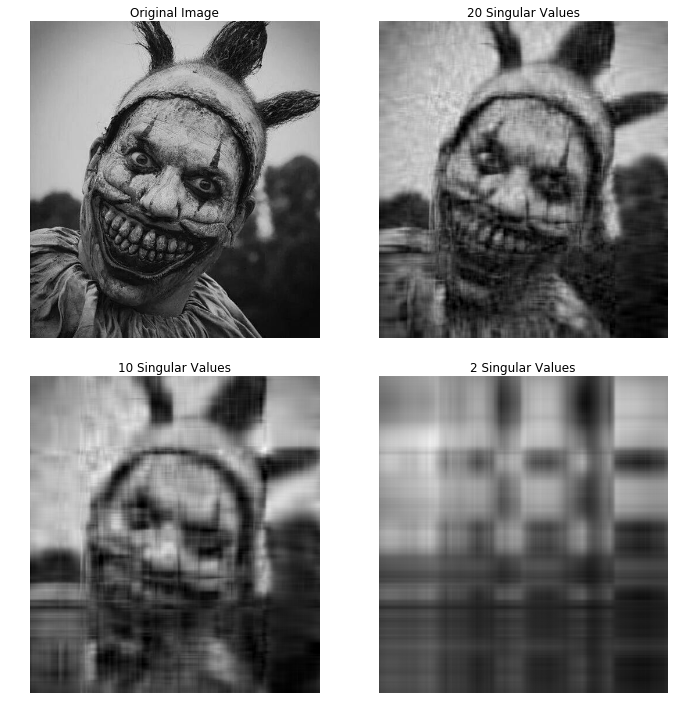
\includegraphics[scale = .5]{p5comp.png}\\\\
The singular values. Note that the original image has many more high singular values, which means it can be compressed effectively using those values. This is a product of the fact that the original image has structure, while the random image does not.\\\\
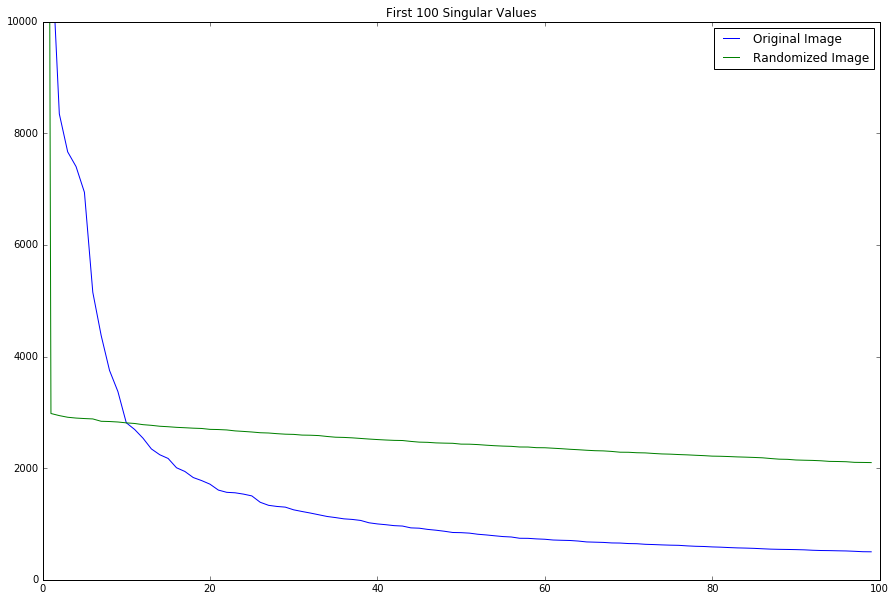
\includegraphics[scale = .5]{p5rand.png}\\\\



\textbf{6. (Murphy 12.5 - Deriving the Residual Error for PCA)} It may be helpful to reference
section 12.2.2 of Murphy.
\begin{enumerate}[(a)]
    \item Prove that
        \[
            \left\|\xx_i - \sum_{j=1}^k z_{ij}\vv_j\right\|^2 = \xx_i^\T\xx_i - \sum_{i=1}^k\vv_j^\T \xx_i\xx_i^\T \vv_j.
        \]
        Hint: first consider the case when $k=2$. Use the fact that $\vv_i^\T\vv_j$ is 1 if $i=j$ and 0 otherwise.
        Recall that $z_{ij} = \xx_i^\T\vv_j$.

    \item Now show that
        \[
            J_k = \frac{1}{n}\sum_{i=1}^n \left(\xx_i^\T \xx_i - \sum_{i=1}^k\vv_j^\T \xx_i\xx_i^\T \vv_j\right) = \frac{1}{n}\sum_{i=1}^n \xx_i^\T\xx_i - \sum_{j=1}^k\lambda_j.
        \]
        Hint: recall that $\vv_j^\T \Sigmab \vv_j = \lambda_j\vv_j^\T\vv_j = \lambda_j$.

    \item If $k=d$ there is no truncation, so $J_d=0$. Use this to show that the error from only using $k<d$
        terms is given by
        \[
            J_k = \sum_{j=k+1}^d \lambda_j.
        \]
        Hint: partition the sum $\sum_{j=1}^d \lambda_j$ into $\sum_{j=1}^k \lambda_j$ and $\sum_{j=k+1}^d \lambda_j$.
\end{enumerate}
\end{document}